\documentclass[10pt]{standalone}
\usepackage{commands}

\begin{document}
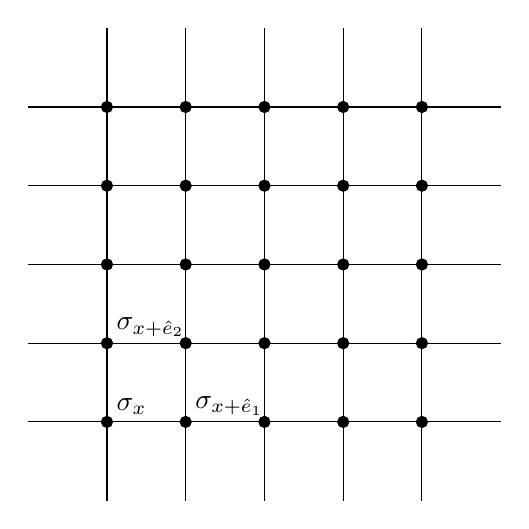
\begin{tikzpicture}
    \foreach \j in {1,...,5} {
            \draw[] (-1, \j) -- (5, \j);
    };
    \foreach \i in {0,...,4} {
        \foreach \j in {1,...,5} {
            \filldraw (\i, \j) circle (2pt);
        }
        \draw[] (\i, 0) -- (\i, 6);
    };
\node[right] at (0, 1.2) {$\sigma_x$};
\node[right] at (1, 1.2) {$\sigma_{x + \hat{e}_1}$};
\node[right] at (0, 2.2) {$\sigma_{x + \hat{e}_2}$};
\end{tikzpicture}
\end{document}